
\begin{document}
\abstract{Balanced Scorecard y Business model canvas son técnicas de análisis empresarial . Ambas técnicas son útiles para mejorar el desempeño organizacional. Pero sus aplicaciones difieren. Ambos se pueden usar junto con los indicadores clave de rendimiento para monitorear y mejorar el rendimiento de la organización. Vamos a entender tanto la técnica en detalle.}

 Abstract\\
Balanced Scorecard and Business model canvas are business analysis techniques. Both techniques are useful to improve organizational performance. But their applications differ. Both can be used together with the key performance indicators to monitor and improve the performance of the organization. We will understand both the technique and the detail.
\newpage

\section{Introduccion}
Esta metodología deriva de la gestión estratégica de empresas y presupone una elección de indicadores que no debe ser restringida al área económico – financiera. Así como no es posible comandar un avión controlando apenas la velocidad, los indicadores financieros no son suficientes para garantizar que una empresa se dirija en la dirección correcta. Por estos motivos, será necesario monitorear, junto a los indicadores económicos –financieros, el desempeño de mercado, los procesos internos, la innovación y la tecnología. De este modo, los resultados financieros serán fruto de la sumatoria de acciones generadas por personas a través del uso de las mejores tecnologías, vinculación a las mejores prácticas y los procesos internos de la organización, todo esto en armoníacon la Propuesta de Valor ofrecida al cliente. Esto proceso se denomina "crear valor através de activos intangibles"

\begin{center}
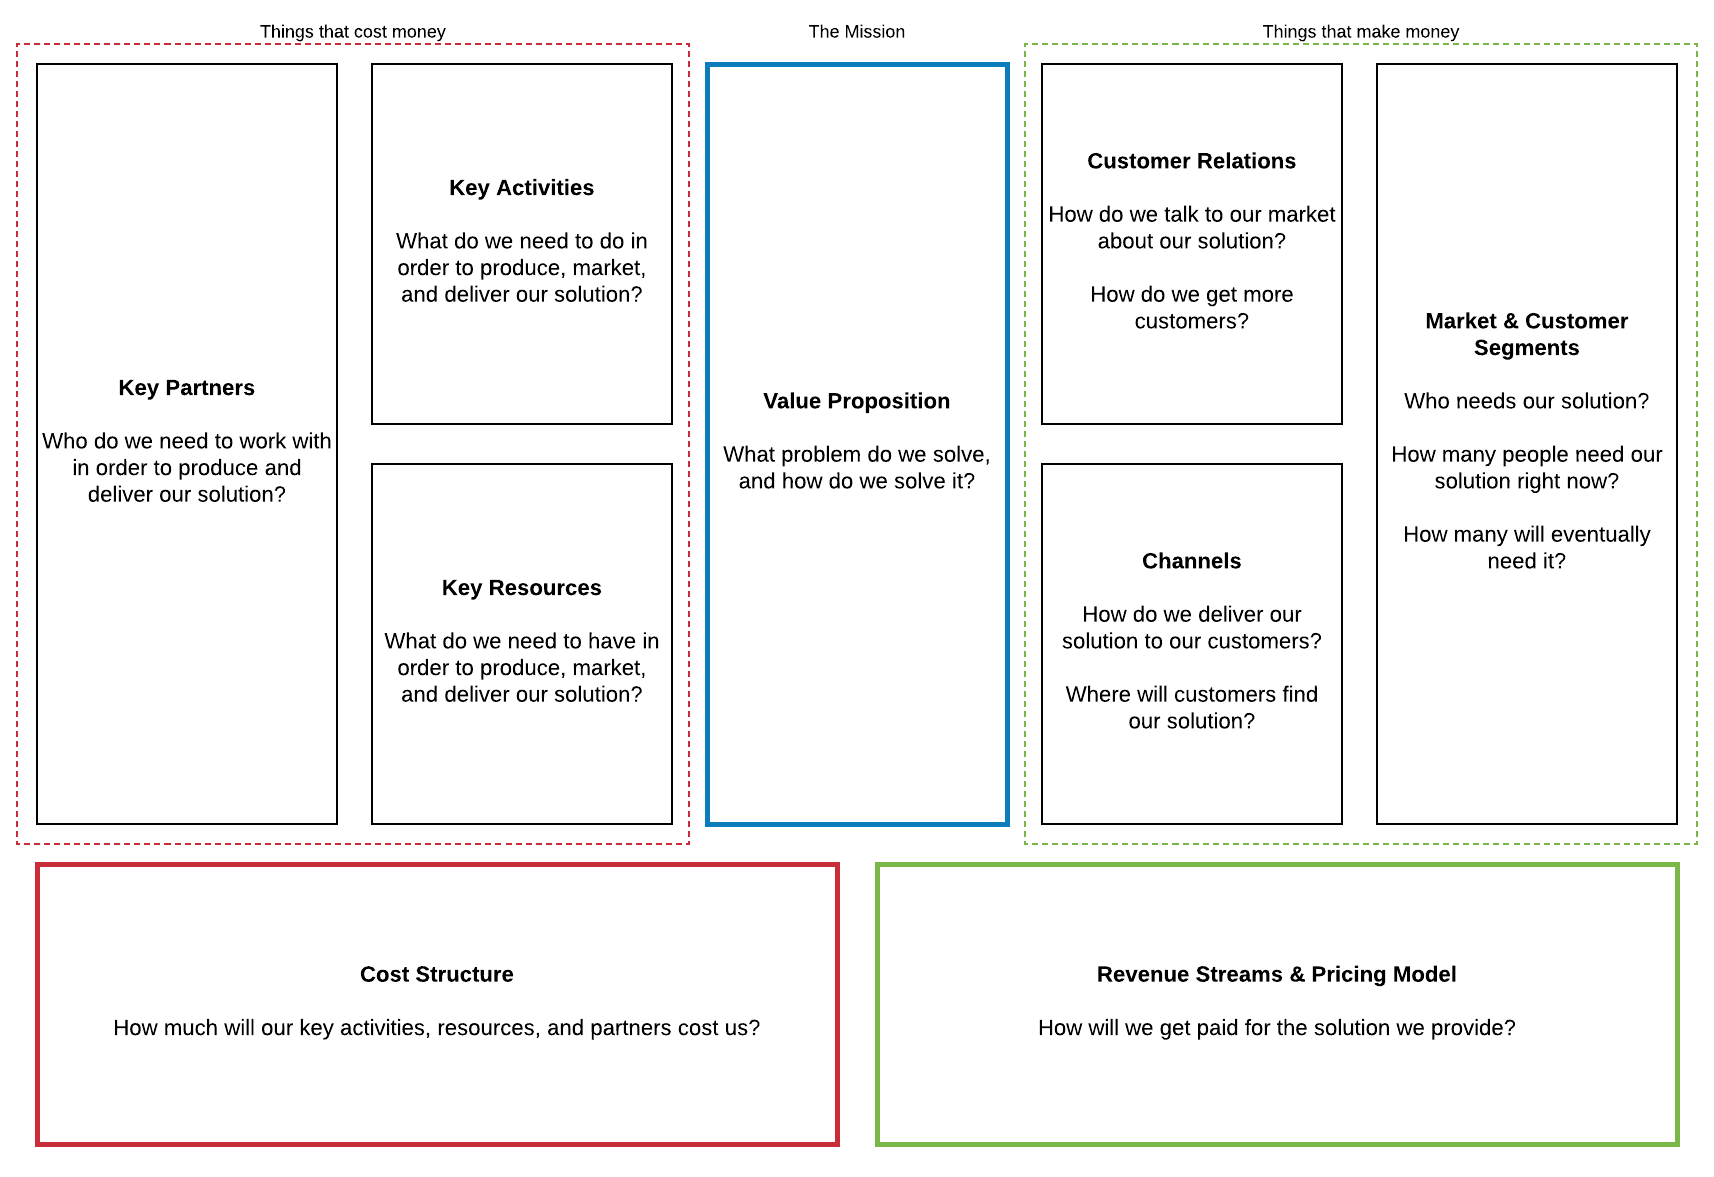
\includegraphics[width=10cm]{./Imagenes/imagen5}
\end{center}

Balanced Scorecard ofrece una visión integrada y balanceada de la empresa y permite desarrollar la estrategia en forma clara. Esto se logra a través de objetivos estratégicos identificados en 4 perspectivas: financiera, clientes, procesos internos yaprendizaje e innovación. Cada una de las perspectivas se vincula con las demás mediante relaciones de causa y efecto. BSC promueve, además, el alineamiento de losobjetivos estratégicos con indicadores de desempeño, metas y planes de acción para hacer posible la generación de estrategias en forma integrada y garantizar que los esfuerzos de la organización se encuentren en línea con las mismas.
\newpage


\section{Balanced Scorecard}
\item{El Balanced Scorecard (BSC) o Cuadro de Mando Integral (CMI) es una herramienta de gestión que permite implementar la estrategia de una empresa a partir de una serie de medidas de actuación, permitiendo un control permanente sobre todos los factores de la organización, interrelacionando objetivos y relacionándolos con acciones concretas.}

\begin{center}
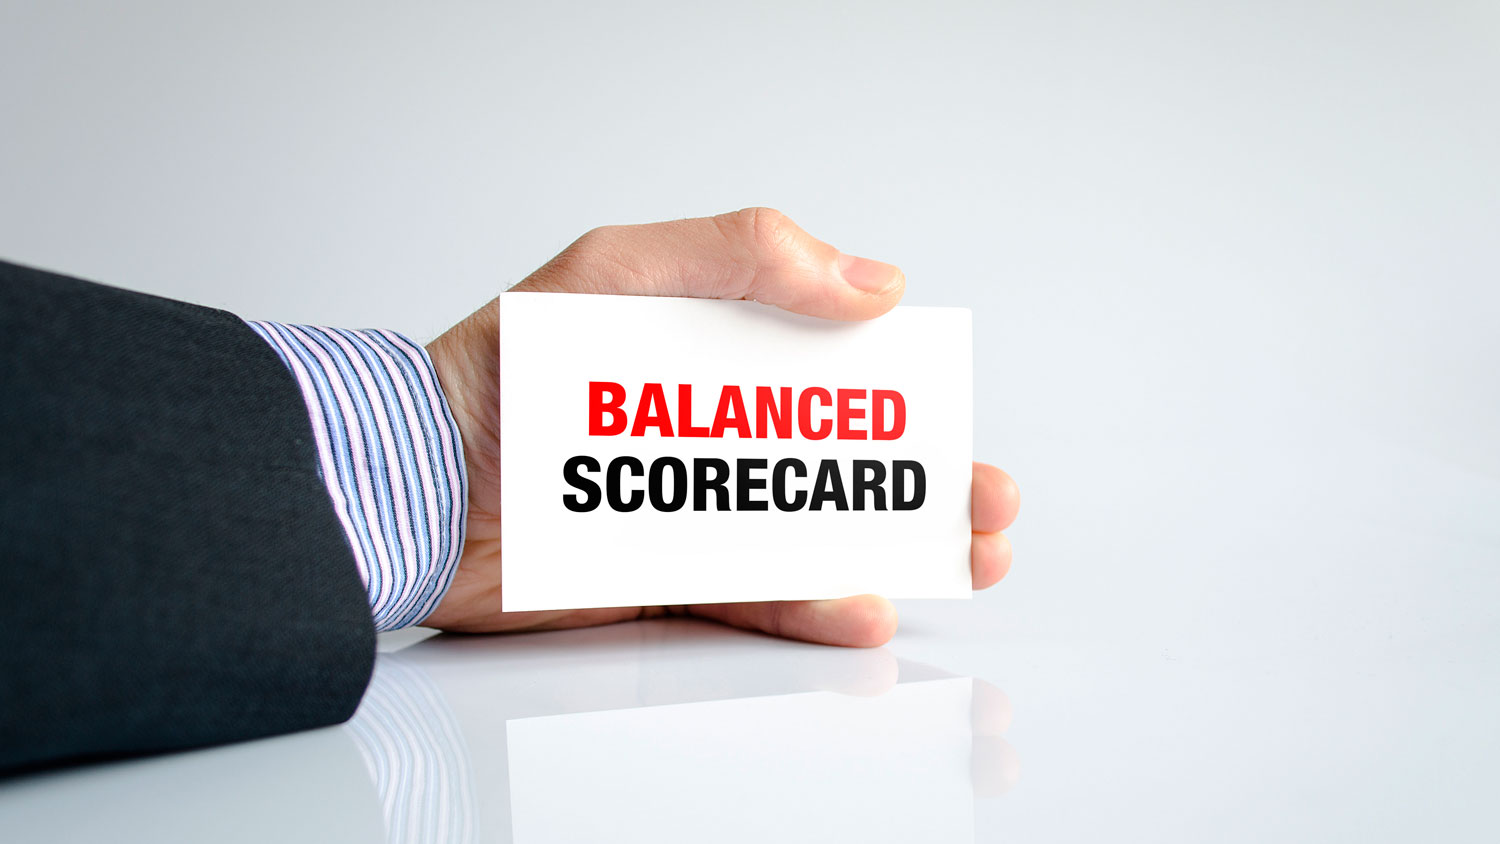
\includegraphics[width=15cm]{./Imagenes/imagen1}
\end{center}

\section{¿Cómo funciona el Balanced Scorecard?}
\item{El proceso de creación de un BSC comienza con la determinación de los siguientes parámetros:\\\\
-Objetivos a alcanzar por la organización.\\
-Indicadores o mediciones más adecuados para poder controlar el grado de alance de los objetivos.\\
-Metas concretas en relación a los resultados específicos de dichas mediciones.\\
-Acciones, iniciativas proyectos o programas que se van a implementar para lograr dichas acciones.\\\\
Una vez fijados todos estos factores, el siguiente paso es colocar todas estas mediciones, metas y objetivos en un panel o cuadro, utilizando para ellos un software específico donde se monitorea el progreso de cada uno de ellos.\\
Los datos, que normalmente se obtienen de los sistemas informáticos de la empresa, se presentan de manera esquemática y muy gráfica en un panel similar al que utilizan los pilotos de aviones, por lo que también se le conoce como «Cuadro de Mando Integral».}

\section{Perspectivas del Balanced Scorecard}
\item{A pesar de que son 4 las perspectivas que tradicionalmente identifican un BSC, no es indispensable que estén todas ellas; estas perspectivas son las más comunes y pueden adaptarse a la gran mayoría de las empresas, y no constituyen una condición indispensable para construir un modelo de negocios.\\\\\

\begin{center}
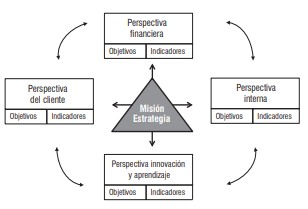
\includegraphics[width=15cm]{./Imagenes/Imagen02}
\end{center}

\textbf{Perspectiva financiera}\\
Históricamente los indicadores financieros han sido los más utilizados, pues son el reflejo de lo que está ocurriendo con las inversiones y el valor añadido económico, de hecho, todas las medidas que forman parte de la relación causa-efecto, culminan en la mejor actuación financiera.Información administrada por un sistema ERP.\\\\
\textbf{Perspectiva del cliente}
Como parte de un modelo de negocios, se identifica el mercado y el cliente hacia el cual se dirige el servicio o producto. La perspectiva del cliente es un reflejo del mercado en el cual se está compitiendo. Brinda información importante para generar, adquirir, retener y satisfacer a los clientes, obtener cuota de mercado, rentabilidad, etc. "La perspectiva del cliente permite a los directivos de unidades de negocio articular la estrategia de cliente basada en el mercado, que proporcionará unos rendimientos financieros futuros de categoría superior." (Kaplan & Norton).
Información administrada por un sistema CRM o BPC.\\\\
\textbf{Perspectiva procesos internos}\\
Para alcanzar los objetivos de clientes y financieros es necesario realizar con excelencia ciertos procesos que dan vida a la empresa. Esos procesos en los que se debe ser excelente son los que identifican los directivos y ponen especial atención para que se lleven a cabo de una forma perfecta, y así influyan a conseguir los objetivos de accionistas y clientes.
Información administrada por un sistema BPC o BPM.\\\\
\textbf{Perspectiva de formación y crecimiento}\\
Es la perspectiva donde más tiene que ponerse atención, sobre todo si piensan obtenerse resultados constantes a largo plazo. Aquí se identifica la infraestructura necesaria para crear valor a largo plazo. Hay que lograr formación y crecimiento en 3 áreas:\\ personas, sistemas y clima organizacional. Normalmente son intangibles, pues son identificadores relacionados con capacitación a personas, software o desarrollos, máquinas e instalaciones, tecnología y todo lo que hay que potenciar para alcanzar los objetivos de las perspectivas anteriores.
Información administrada por un sistema ERP o BPC.}

\begin{center}
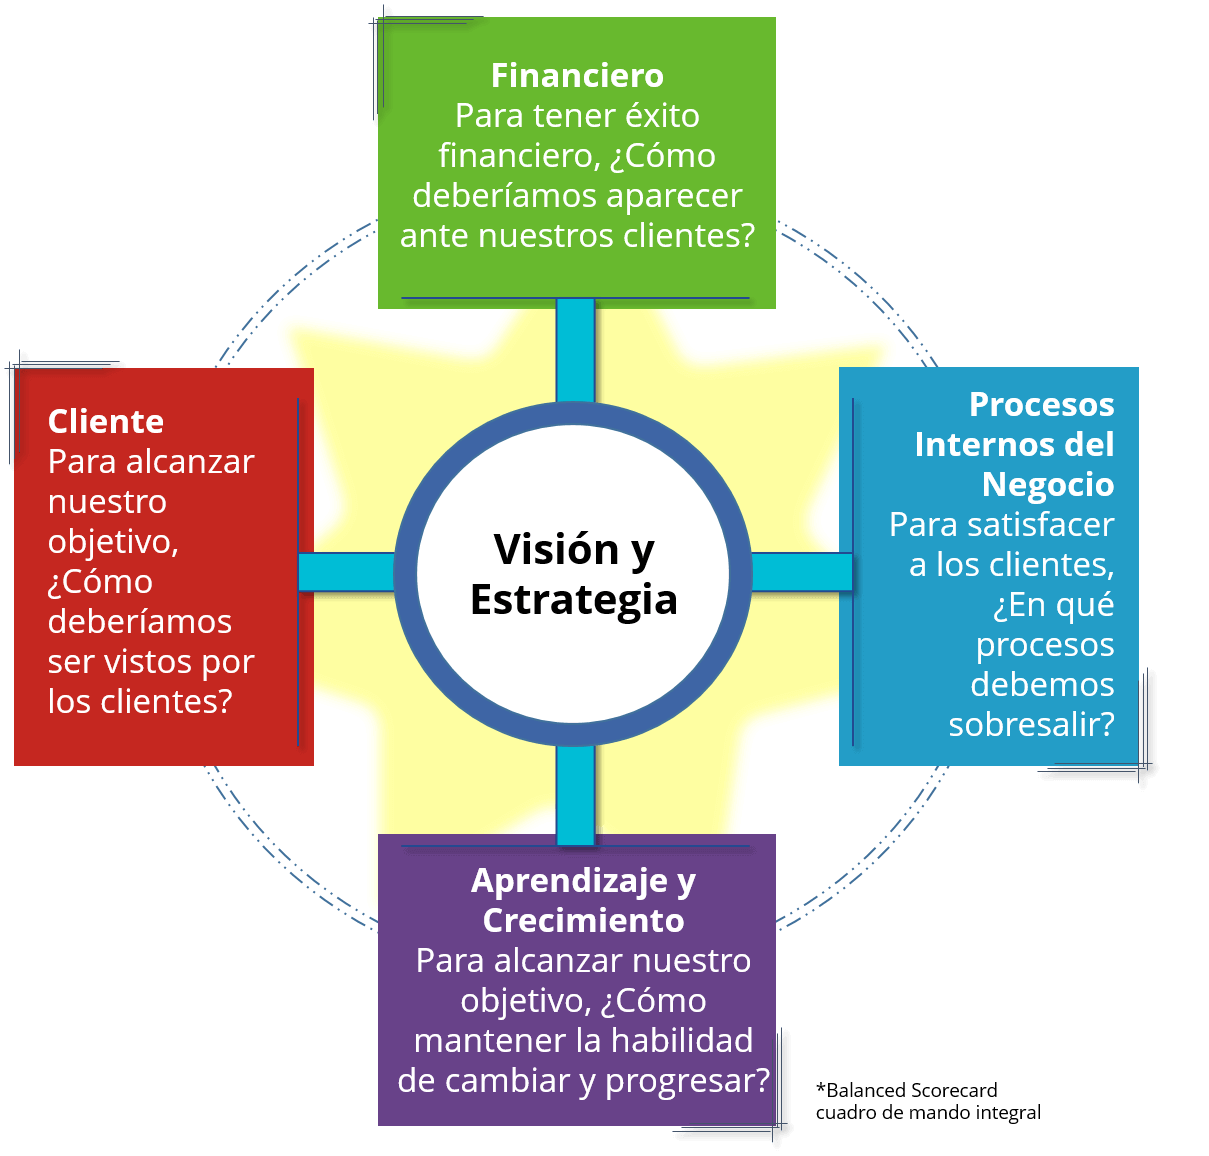
\includegraphics[width=15cm]{./Imagenes/imagen2}
\end{center}

\section{Beneficios}
\item{El Balanced Scorecard induce una serie de resultados que favorecen la administración de la compañía, pero para lograrlo es necesario implementar la metodología y la aplicación para monitorear, y analizar los indicadores obtenidos del análisis. Entre otros podemos considerar las siguientes ventajas:\\\\
-Alineación de los empleados hacia la visión de la empresa.\\
-Comunicación hacia todo el personal de los objetivos y su cumplimiento.\\
-Redefinición de la estrategia en base a resultados.\\
-Traducción de la visión y estrategias en acción.\\
-Favorece en el presente la creación de valor futuro.\\
-Integración de información de diversas áreas de negocio.\\
-Capacidad de análisis.\\
-Mejoría en los indicadores financieros.\\
-Desarrollo laboral de los promotores del proyecto.}

\begin{center}
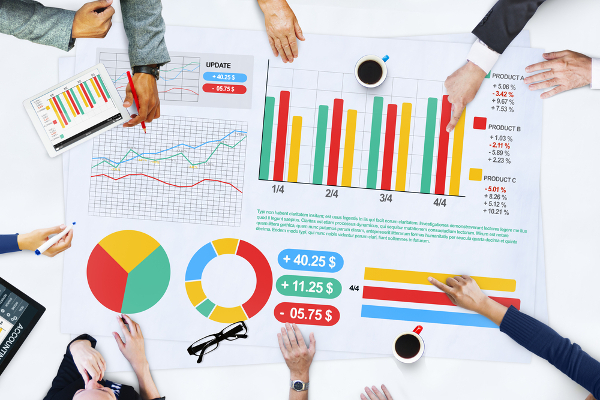
\includegraphics[width=15cm]{./Imagenes/imagen3}
\end{center}

\section{Plan Estrategico}
\item{Es un proceso sistematico de desarrollo e implementacion de planes para alcanzar metas, propositos y objetivos.}

\item{ y debe:}
- Ser capaz de alcanzar el objetivo deseado
- Factible apropiada
- Debe proporcionar una ventaja compettitiva
- Capaz de adaptar a las situciones cambiantes
- Medible en terminos de su efectividad

\section{Modelo Canvas}
\item{
El modelo canvas es la herramienta para analizar y crear modelos de negocio de forma simplificada. Se visualiza de manera global en un lienzo dividido en los principales aspectos que involucran al negocio y gira entorno a la propuesta de valor que se ofrece.\\\\
El modelo canvas se utiliza para pasar de idea a proyecto y plasmar nuestra idea en un modelo empresarial. Es un modelo “vivo”, es decir, que vamos modificando según se va desarrollando, vamos validando clientes, surgen nuevas ideas… por eso se utilizan post-its para completarlo.
}

\section{Generar un modelo canvas}
\item{
Muestra de manera lógica la interconexión entre los 9 aspectos básicos de un modelo de negocio. A continuación, mostramos cómo se debe completar un modelo canvas, en qué orden y qué significa cada apartado del lienzo.\\\\
\textbf{1. Segmento de clientes}\\
Detectar las necesidades del mercado, del cliente. Nuestro foco siempre es el cliente y debemos orientar el producto a sus necesidades y deseos.\\
Para poder identificar a nuestro cliente debemos ponernos en su piel y analizar qué es lo que piensa, siente, ve, escucha, cuáles son sus problemas y los beneficios que le puede aportar nuestro producto/servicio.\\\\
Debemos dar respuesta a:\\
¿Para quién estamos creando valor?\\
¿Quiénes son nuestros clientes más importantes?
\\\\\textbf{2. Propuesta de valor}\\
Es la pieza clave de todo el modelo de negocio. La propuesta de valor o ventaja competitiva es el motivo por el que el cliente nos va a comprar a nosotros y no a otro. Aquí se incluye lo que hace diferente e innovador a nuestro producto/servicio.\\
Se puede innovar en diferentes aspectos como en el modelo de ingresos, alianzas empresariales, procesos productivos, entrega del producto/servicio, marca…\\\\
Debemos dar respuesta a:\\
¿Qué valor estamos entregando a nuestros clientes?\\
¿Qué problema resolvemos?\\
¿Cuál es la necesidad que satisfacemos?\\
¿Qué tipo de producto ofrecemos?\\\\
\textbf{3. Canales}\\
Una vez definidos nuestros clientes y la propuesta de valor que les ofrecemos, tenemos que llegar a ellos. Si no nos conocen, no nos van a comprar. Aquí vamos a definir los canales de distribución del producto o servicio.\\\\
Debemos dar respuesta a:\\
¿Con qué canales podemos llegar a nuestros clientes?\\
¿Qué canales funcionan mejor?\\
¿Cuáles de estos canales son los más rentables?\\\\
\textbf{4. Relación con los clientes}\\
Debemos comunicarnos correctamente con nuestros clientes y estar pendiente de ellos. Ellos son nuestro eje central, por lo que saber definir la relación que vamos a tener con cada segmento de clientes, es fundamental para el éxito de un negocio.\\\\
Debemos dar respuesta a:\\
¿Cuál es la relación que tenemos con cada uno de nuestros segmentos de clientes?\\
¿Qué tipo de relación esperan?\\
¿Qué coste tiene?\\\\
\textbf{5. Flujo de ingresos}\\
Para que un negocio sea rentable y podamos sobrevivir en el mercado, tenemos que pensar ¿Cómo monetizarlo? Es decir ¿De dónde vamos a obtener la facturación?\\\\
Debemos dar respuesta a:\\
¿Cuál es nuestra principal línea de ingresos? \\
¿Cómo pagarán nuestros clientes?\\
¿Por qué están dispuestos a pagar nuestros clientes?\\\\
\textbf{6. Recursos clave}
Conocer con qué recursos contamos y con los que debemos contar para llevar a cabo la actividad de nuestro negocio, es clave a la hora de establecer el plan de negocios. Debemos de ser cautos y prudentes a la hora de definir estos recursos. Siempre debemos pensar en la forma de optimizarlos, es decir, intentar conseguir la máxima productividad posible al mínimo coste.\\\\
Debemos dar respuesta a:\\
¿Qué recursos esenciales requiere nuestra propuesta de valor?\\\\
\textbf{7. Actividades clave}\\
Para llevar a cabo la propuesta de valor que queremos ofrecer a nuestros clientes, son necesarias ciertas actividades para preparar el producto antes de que llegue al mercado. Es decir, aquí pensamos en el core de nuestro negocio, lo que haremos en nuestro día a día.\\\\
Debemos dar respuesta a:\\
¿Qué actividad básica requiere nuestra propuesta de valor?\\
¿Cuáles son nuestros canales?\\
¿Cuáles son nuestras fuentes de ingresos?\\\\
\textbf{8. Aliados clave}\\
Para llevar a cabo un negocio, es imprescindible tener aliados. Estos aliados pueden ser;\\\\
Una serie de socios/colaboradores: una buena red de partners nos pueden ayudar a llegar más rápido al cliente, a ir avalados por su reputación y experiencia.\\
Los proveedores: aquellos que nos proporcionan los recursos clave para poder ofrecer los servicios/producto final.\\\\
Debemos dar respuesta a:\\
¿Quiénes son nuestros socios clave en el mercado?\\
¿Quiénes son nuestros proveedores?\\
\textbf{9. Estructura de costes}\\
Obviamente, toda esta infraestructura tiene unos costes que debemos pagar y optimizar. Debemos definir cuáles son nuestras prioridades y los gastos fundamentales en el negocio de aquellos que no lo son.\\
Tener bien clara esta estructura nos ayudará a no desviarnos de los presupuestos y que el negocio fracase por problemas de financiación.\\\\
Debemos dar respuesta a:\\\\
¿Cuáles son los costes más importantes dentro de nuestro modelo de negocio?\\
¿Qué recursos clave son los más costosos?\\
¿Qué actividades clave son las más costosas?\\
}
\begin{center}
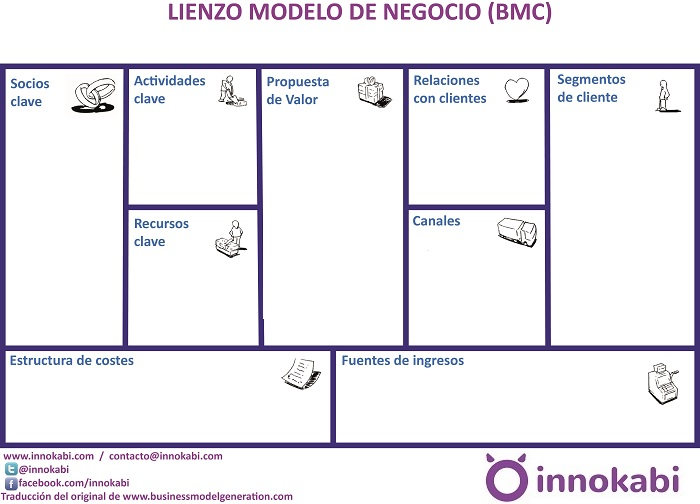
\includegraphics[width=15cm]{./Imagenes/imagen4}
\end{center}


\title{BALANCED SCORECARD EJEMPLO DE IMPLEMENTACIÓN EN UNA CORPORACIÓN EDITORIAL PARA MANTENER UNA POSICIÓN DE LIDERAZGO EN EL MERCADO}

\section{ANTECEDENTES Y JUSTIFICACIONES}
\item { Grupo Santillana Ecuador es una empresa de capitales españoles que ha liderado el sector editorial de texto escolar en Ecuador por los últimos 10 años. En este tiempo, se ha consolidado como la primera opción en el mercado escolar de textos de prescripción.

También ha logrado incursionar en nuevas unidades de negocios en los cuales tiene una participación representativa en el mercado nacional entre las que se destacan la comercialización de textos literarios para el público en general y servicios de capacitación a nivel de postgrado.}

\section{Su Estructura Comercial está conformada por cuatro líneas de negocio:}
\item { 1.-  Texto Escolar: es el sello con el cual edita y difunde textos y materiales para educación escolar.

2.- Richmond (Inglés): es el sello encargado de desarrollar y comercializar material didáctico para la enseñanza del idioma inglés para educación escolar.

3.- Ediciones Generales: comercializa libros de diversos sellos literarios que llegan al público lector para satisfacer la demanda de gran variedad de temas.

4.- Santillana Formación:  Es una nueva unidad de negocio que se divide en dos líneas de servicios:

1. Instituto Universitario de Postgrados – IUP: Convenio con universidades españolas que le acredita a Santillana desarrollar programas de postgrados que permitan a profesionales ecuatorianos acceder a maestrías internacionales.

2. Santillana Profesional: diseño de proyectos educativos mediante modernas tecnologías (e – learnig).}

\begin{center}
\includegraphics[width=15cm]{./Imagenes/ImgEmpresa1.png}
\end{center}

\item { A pesar del éxito obtenido en los últimos años, Santillana ha visto la necesidad de buscar nuevas estrategias y mecanismos de gestión  para mantener esa posición de liderazgo frente a la creciente y agresiva competencia en todas sus líneas de negocio.

Especialmente en la que consideran su bastión, texto escolar, que constantemente se ve amenazado por empresas rivales que copian y anulan muchas de las estrategias comerciales implementadas.}

\section{BALANCED SCORECARD EJEMPLO DE HERRAMIENTA: POR QUÉ RAZÓN ELIGIERON USAR UN TABLERO DE COMANDO}
\item { Con este antecedente y luego que a finales del 2004 se definiera el Plan Estratégico de la organización que contempla objetivos claves que deben cumplirse hasta el año 2009, se decidió implementar una herramienta de control estratégico como el BSC para darle seguimiento a la estrategia, y proyectos para cumplir los propósitos establecidos.

En este proceso, surgió la pregunta ¿Cómo hacer para que los planes de la Organización dejen de ser planes y se conviertan en realidad?

El primer paso para responder a esta pregunta es tener en cuenta que los activos intangibles conforman el mayor valor de toda Organización y que ninguna estrategia daría resultados positivos si no se le da el seguimiento apropiado.

Se decidió utilizar el Balance Scorecard debido a los beneficios que proporciona involucrando a los activos intangibles con su relación de desempeño. Además que el rápido retorno de la inversión estimada inclinaban ciertamente la utilización de esta herramienta.

Se estimó que luego de la implementación, cuando esté en explotación todo el sistema, los logros que se obtengan motivarán a seguir realizando nuevas mejoras en la organización. Con ello, a más darle seguimiento a la estrategia y de lograr un retorno de la inversión en un corto plazo, se logran fortalecer algunas debilidades que se identificaron en la empresa. Entre las más destacables:

1. Mejorar el sistema de comunicación interno
2. Disciplinar al personal
3. Crear cultura de medición y consecución de objetivos.
4. Establecer mecanismos de retroalimentación para mejoras

Otro factor que influyó en tomar la decisión de utilizar el Scorecard como herramienta de gestión estuvo relacionado con la administración y seguimiento de las diversas áreas de negocios con las que cuenta actualmente la empresa.

En vista de que se cuenta con cuatro unidades de negocios, 3 de ellas bien diferenciadas, se estableció como necesidad delinear estrategias distintas y segmentadas para cada una de ellas, las mismas que se deberían estar alineadas con la estrategia corporativa global de crecimiento financiero fijada por la matriz.}

\section{BALANCED SCORECARD EJEMPLO DE IMPLEMENTACIÓN}
\item {El proceso de implementación en Grupo Santillana inició luego de validar  el plan estratégico acordado hasta el 2009, y se estableciera un ROADMAP a seguir para cubrir la brecha entre la situación actual y la deseada en ese umbral de tiempo.

En este mapa de camino, se establecen claramente los pasos a seguir y nos da un estimado de tiempo para su consecución (un mes por cada uno de las fases):}

\begin{center}
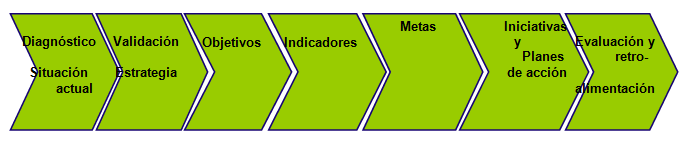
\includegraphics[width=15cm]{./Imagenes/ImagenEmpresa2.png}
\end{center}

\section{BALANCED SCORECARD EJEMPLO DE IMPLEMENTACIÓN}
\item {El proceso de implementación en Grupo Santillana inició luego de validar  el plan estratégico acordado hasta el 2009, y se estableciera un ROADMAP a seguir para cubrir la brecha entre la situación actual y la deseada en ese umbral de tiempo.

En este mapa de camino, se establecen claramente los pasos a seguir y nos da un estimado de tiempo para su consecución (un mes por cada uno de las fases):}

\section{Balanced Scorecard Ejemplo de Implementación – Paso 1}
\item {Definir el Mapa Estratégico Corporativo y Validación de la Estrategia

Clarificar la Visión definida por la empresa en el Plan Estratégico fue la primera de las actividades realizadas, debido a que de ahí se derivan el resto de componentes del scorecard.

Formular la hipótesis estratégica (seleccionar los temas estratégicos) se hizo conjuntamente con la validación de la visión de la empresa y surgieron algunas dudas que se fueron aclarando y puliendo hasta obtener el cuadro de mando corporativo, que sería la base de nuestro scorecard.

Esta estrategia global fue “bajada” a un segundo nivel para trabajarla por cada unidad de negocio, por lo que cada unidad trabajó en su propuesta de valor única para su segmento específico de clientes, con los cuales se desarrollo esa combinación de producto, calidad de servicio, precio, e imagen que se ofrece a los clientes para distinguirse de la competencia.

El cuadro de mando para Santillana se lo trabajó en 2 niveles de los 3 posibles, al nivel gerencial o mandos altos, y al nivel de mandos medios, se dejó de lado por esta ocasión el cascadearlo hasta el nivel operativo por motivo de recursos y tiempo. Sin embargo, existe la intención de abarcar este nivel en un futuro cercano una vez que el esquema de remuneración variable también sea habilitado.

El mapa aquí presentado es claro y nos demuestra las relaciones causa y efecto entre cada perspectiva, tratando de armonizar con el cuadro de mando que se maneja bajo la misma filosofía, dado que no es posible buscar las respuestas al desempeño financiero en la misma perspectiva sino en su concatenación con el resto de áreas que directamente influyen en esos resultados. El objetivo fue no perder el concepto de integralidad.}

\begin{center}
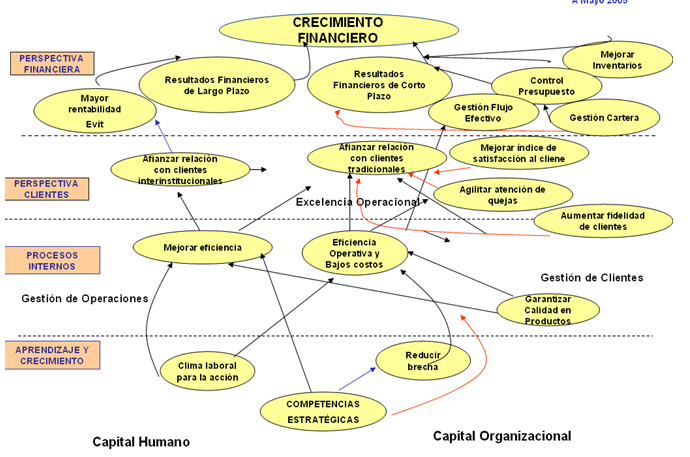
\includegraphics[width=15cm]{./Imagenes/ImagenEmpresa3.png}
\end{center}

\section{Balanced Scorecard Ejemplo de Implementación – Paso 2: Objetivos Estratégicos Corporativos por Perspectiva}
\item {1. Se trabajó en establecer “Propuesta de Valor” por cada segmento de clientes. Entre los cuales deberíamos diferenciar por unidad de negocio, por estrato social y por capacidad de consumo. En todos ellos se acordó que la propuesta ganadora estaría principalmente enfocada en tener una mayor intimidad con el cliente, para conocerlo mejor y de esa forma poder adaptar nuestra oferta a sus gustos.

2. Definir los objetivos de contribución para cada perspectiva y objetivos estratégicos establecidos.  Este fue un factor importantísimo dado que con cada gerente de área se trabajo detenidamente para determinar en qué forma su área podía alinearse con los objetivos estratégicos corporativos ya definidos. Se lograron importantes análisis que se incluyeron como aportes de cada área, los cuales fueron luego llevados a iniciativas y planes de acción.

3. Identificación de los procesos de gestión críticos para alcanzar la estrategia
Se identificaron cuales procesos se consideraban críticos para alcanzar lo propuesto, luego de varias charlas y análisis conjunto entre los gerentes de área, se acordó que implementar un sistema de control y atención de quejas y otro de información para fidelidad y retención.

Para ayudarnos a identificar estos procesos se recurrió muchas veces a sencillas preguntas como:

* Qué necesidades de información no han sido satisfechas
* Por qué hacemos las cosas de esta forma y no de otra
* Qué vacíos encontramos en los procesos actuales
* Por qué no hemos enfrentado este problema con anterioridad
* Cómo podemos mejorar esa área
* Qué necesitamos para fortalecer nuestras debilidades
* Qué se nos pasó por encima.}


% Bibliografía.
%-----------------------------------------------------------------
\begin{thebibliography}{99}
https://www.isotools.org/2015/02/23/que-es-el-balanced-scorecard-conoce-su-funcionamiento-y-ventajas/\\
https://economipedia.com/definiciones/modelo-canvas.html\\
http://www.infoviews.com.mx/Bitam/ScoreCard/]\\
https://innokabi.com/canvas-de-modelo-de-negocio/\\
https://josefacchin.com/modelo-canvas-de-negocio/\\
https://www.adaptiveus.com/balanced-scorecard-vs-business-model-canvas/\\

\bibitem{Cd94} Autor, \emph{Título}, Revista/Editor, (año)

\end{thebibliography}

\end{document}
